%\documentclass[showpacs,preprintnumbers,amsmath,amssymb,superscriptaddress,aip]{revtex4-1}
\documentclass[letter,scriptaddress,twocolumn, prl,showkeys]{revtex4}
\usepackage{graphicx}
%\setlength{\parindent}{0in}

% General Latex  --------------------------------------------------
\def\beq{\begin{equation}}
\def\eeq{\end{equation}}
\def\beqar{\begin{eqnarray}}
\def\eeqar{\end{eqnarray}}
\def\nn{\nonumber}
\def\ol{\overline}
\def\para{\parallel}

% Operators  ------------------------------------------------------
\newcommand{\diff}[2]{\frac{d#1}{d#2}}
\newcommand{\diffs}[2]{\frac{d^2#1}{d#2^2}}
\newcommand{\pdiff}[2]{\frac{\partial#1}{\partial#2}}
\newcommand{\pdiffs}[2]{\frac{\partial^2#1}{\partial#2^2}}
\newcommand{\pdiffxy}[3]{\frac{\partial^2#1}{\partial#2 \partial#3}}
\newcommand{\pdt}{\partial_t}
\newcommand{\pdr}{\partial_r}
\newcommand{\pdth}{\partial_\theta}
\newcommand{\pdrr}{\partial^2_r}

\newcommand{\enum}[2]{{#1}\times10^{#2}} % 4.2x10^{3} = \enum{4.2}{3}

\newcommand{\vect}[1]{{\bf #1}}
%\newcommand{\vect}{\overrightarrow}
%\newcommand{\vect}{\vec}
\def\div{\nabla\cdot}
\def\grad{\nabla}
\def\curl{\nabla\times}
\newcommand{\gradpar}{\grad_\parallel}
\newcommand{\gradperp}{\grad_\perp}
\newcommand{\gradr}{\grad_r}
\newcommand{\defeq}{\ensuremath{\stackrel{\text{\tiny def}}{=}}}

\newcommand{\savg}[1]{\left<{#1}\right>}
\newcommand{\vavg}[1]{\left<{#1}\right>_V}
\newcommand{\thavg}[1]{\left<{#1}\right>_\theta}

% Variable names  -------------------------------------------------
\newcommand{\vpar} {v_\parallel}
\newcommand{\Apar} {A_\parallel}
\newcommand{\jpar} {j_\parallel}
\newcommand{\kpar} {k_\parallel}
\newcommand{\kperp} {k_\perp }
\newcommand{\vperp} {v_\perp }
\newcommand{\kthe}{k_\theta}

\newcommand{\Evec}{\ensuremath{\boldsymbol{{\rm E}}}}
\newcommand{\Bvec}{\ensuremath{\boldsymbol{{\rm B}}}}
\newcommand{\Jvec}{\ensuremath{\boldsymbol{{\rm J}}}}
\newcommand{\Fvec}{\ensuremath{\boldsymbol{{\rm F}}}}
\newcommand{\fvec}{\ensuremath{\boldsymbol{{\rm f}}}}
\newcommand{\vE}{\ensuremath{\boldsymbol{{\rm v}_{E}}}}
\newcommand{\bo}{\ensuremath{\boldsymbol{{\rm b}_0}}}
\newcommand{\bvec}{\ensuremath{\boldsymbol{{\rm b}}}}
\newcommand{\xvec}{\ensuremath{\boldsymbol{{\rm x}}}}
\newcommand{\yvec}{\ensuremath{\boldsymbol{{\rm y}}}}
\newcommand{\zvec}{\ensuremath{\boldsymbol{{\rm z}}}}
\newcommand{\vvec}{\ensuremath{\boldsymbol{{\rm v}}}}
\newcommand{\jvec}{\ensuremath{\boldsymbol{{\rm j}}}}

\newcommand{\bxgp}{\bvec\times\gradperp}

\newcommand{\vve}{\ensuremath{\boldsymbol{{\rm v}}_{e}}}
\newcommand{\vvi}{\ensuremath{\boldsymbol{{\rm v}}_{i}}}
\newcommand{\vpe}{v_{\parallel e}}
\newcommand{\vpi}{v_{\parallel i}}
\newcommand{\vvE}{\ensuremath{\boldsymbol{{\rm v}}_{E}}}
\newcommand{\vvD}{\ensuremath{\boldsymbol{{\rm v}}_{D}}}

\newcommand{\nuei}{\nu_{ei}}
\newcommand{\nuii}{\nu_{ii}}
\newcommand{\nue}{\nu_{e}}
\newcommand{\nuen}{\nu_{en}}
\newcommand{\nuin}{\nu_{in}}
\newcommand{\kpe}{\kappa_{\parallel e}}

\newcommand{\rs}{\rho_{s}}
\newcommand{\ri}{\rho_{i}}
\newcommand{\wci}{\Omega_{i}}
\newcommand{\wcix}{\Omega_{ix}}
\newcommand{\wce}{\Omega_{e}}
\newcommand{\tomega}{\tilde\omega}
\newcommand{\Isat}{I_{\rm sat}}
\newcommand{\fmie}{\frac{m_i}{m_e}}
\newcommand{\fmei}{\frac{m_e}{m_i}}


% Often used dimensions
\newcommand{\cm}{\rm cm}
\newcommand{\mm}{\rm mm}
\newcommand{\cmn}{{\rm cm}^{-3}}
\newcommand{\mn}{{\rm m}^{-3}}
\newcommand{\eV}{\rm eV}
\newcommand{\G}{\rm G}
\newcommand{\T}{\rm T}



\begin{document}

\title{A Linear Technique to Predict Non-Normal Turbulence Applied to a Magnetized Plasma}

\author{B. Friedman}
\email{friedman@physics.ucla.edu}

\author{T.A. Carter}

\affiliation{Department of Physics and Astronomy, University of California, Los Angeles, California 90095-1547, USA}



\begin{abstract}
In nonlinear dynamical systems with highly nonorthogonal linear eigenvectors, linear non-modal analysis is more useful than normal mode analysis in predicting turbulent properties. 
However, the non-trivial time evolution of non-modal structures makes quantitative prediction difficult. We present a technique to overcome this difficulty by modelling the effect that the advective nonlinearities have on spatial turbulent structures. The nonlinearities are taken as a periodic randomizing force with
period consistent with critical balance arguments. We apply this technique to a model of drift wave turbulence in the Large Plasma Device (LAPD) 
[W. Gekelman \emph{et al.}, Rev. Sci. Inst. {\bf 62}, 2875 (1991)], where non-modal effects dominate the turbulence.
We compare the resulting growth rate spectrum to that obtained from a nonlinear simulation, showing good quantitative agreement.
\end{abstract}

\maketitle

Normal mode analysis -- the calculation of eigenvalues and eigenvectors of a linearized dynamical system -- has been used to solve many problems over the years.
Despite its wide-ranging success, it has failed in important instances, particularly in predicting the onset of subcritical turbulence in hydrodynamic flows. 
The reason for this failure was explained in the early 1990's when Trefethen and others attributed the pitfalls of normal mode analysis to the non-normality of linear operators of
dynamical systems~\cite{trefethen1993,schmid2007}. A non-normal operator has 
eigenvectors that are nonorthogonal to one another. One consequence of eigenvector nonorthogonality is that even when all eigenvectors decay exponentially under linear evolution, 
superpositions of eigenvectors can grow, albeit transiently.
In other words, certain fluctuations of the laminar state can access free energy from background gradients even though normal mode fluctuations cannot.
When combined with nonlinear effects, this allows for sustained subcritical turbulence.
Such behavior is obscured by traditional normal mode analysis, which only effectively describes the long time asymptotic behavior of fluctuations under the 
action of the linear operator. Transient growth events, which can dominate nonlinear evolution, require initial-value (non-modal) calculations rather than normal mode calculations.

Non-modal analysis has been embraced by the hydrodynamics community over the past two decades in the attempt to explain and predict subcritical turbulence. But the plasma community
still heavily relies on normal mode analysis to inform turbulent predictions and observations, with a few notable exceptions~\cite{camargo1998,camporeale2010,schekochihin2012}. 
Furthermore, non-modal treatments have generally been explanatory rather than predictive and have centered around the transition to turbulence in subcritical systems rather 
than on properties of fully-developed turbulence.
This paper takes up the task of developing a quantitative approach to predicting turbulent properties using only non-modal linear calculations. 
Our approach is to evolve the linear solution from an ensemble of random initial conditions 
and calculate the average growth rate of the solutions over a specified timescale.  Optimally this time scale would be the
nonlinear decorrelation time of the turbulent system, but in order to enable predictive capability, we employ critical balance
arguments to use a characteristic \emph{linear} time.
This procedure produces an effective growth rate spectrum that can be used to predict turbulent properties such as saturation levels.
While the concepts behind this technique are general enough to be applied to many nonlinear dynamical systems, the details vary for each case, 
so we restrict our treatment to one particular turbulence model. For this model, the technique reproduces the turbulent growth rate spectrum of the direct nonlinear simulation fairly well, especially
in comparison to the linear eigenmode spectrum.

The model describes pressure-gradient-driven turbulence in the uniformly magnetized, cylindrical plasma
produced by the Large Plasma Device (LAPD)~\cite{gekelman1991}. 
Due to LAPD's large size and high collisionality, a fluid model is
appropriate to describe the turbulence~\cite{Popovich2010a,Popovich2010b,Umansky2011}. We use a reduced Braginskii 2-fluid model:

\beqar
\label{ni_eq}
\pdt N = - {\mathbf v_E} \cdot \grad N_0 - N_0 \gradpar \vpe + S_N + \{\phi,N\}, \\
\label{ve_eq}
\pdt \vpe = - \fmie \frac{T_{e0}}{N_0} \gradpar N - 1.71 \fmie \gradpar T_e  \nonumber \\
+ \fmie \gradpar \phi - \nue \vpe + \{\phi,\vpe \}, \\
\label{rho_eq}
\pdt \varpi = - N_0 \gradpar \vpe  - \nuin \varpi + \{\phi,\varpi \}, \\
\label{te_eq}
\pdt T_e = - {\mathbf v_E} \cdot \grad T_{e0} - 1.71 \frac{2}{3} T_{e0} \gradpar \vpe \nonumber \\
+ \frac{2}{3 N_0} \kpe \gradpar^2 T_e  - \frac{2 m_e}{m_i} \nue T_e  +  S_T + \{\phi,T_e\},
\eeqar
where $N$ is the density, $\vpe$ the parallel electron velocity, $\varpi \equiv \gradperp \cdot (N_0 \gradperp \phi)$ the potential vorticity,
and $T_e$ the electron temperature. All lengths are
normalized to the ion sound gyroradius $\rho_s$, times to the ion cyclotron time $\omega_{ci}^{-1}$, velocities to the sound speed $c_s$, densities to the equilibrium peak density, and electron
temperatures and potentials to the equilibrium peak electron temperature. The profiles $N_0$ and $T_{e0}$ and other parameters are taken from experimental 
measurements~\cite{schaffner2012,friedman2012b,friedman2013}. 
%$\phi_0$  is absent in the equations because we model one particular experiment in which the equilibrium radial electric field was reduced to near zero value using a limiter biasing technique~\cite{schaffner2012}. 

The equations are global and partially linearized. The only nonlinearities retained are the advective nonlinearities, which are written with Poisson brackets. 
We add artificial diffusion and viscosity terms with small numerical coefficients ($10^{-3}$)
to ensure numerical stability in nonlinear simulations, which are performed with the BOUT++ code~\cite{dudson2009}. We use periodic axial and zero value radial 
boundary conditions. Further details of the model, including validation studies, may be found in the references~\cite{Popovich2010a,Popovich2010b,Umansky2011,friedman2012b,friedman2013},
though we mention here that the model does very well in reproducing
the statistical properties of the experimentally-observed turbulence.

The nonlinear simulation reveals a fascinating property of the turbulence -- 
it is dominated by a nonlinear instability process despite being linearly unstable to drift waves~\cite{friedman2012b,friedman2013}.
This nonlinear instability process, which was discovered by Drake et al.~\cite{drake1995} in a similar plasma model, works as follows: 
magnetic-field-aligned ($k_\para=0$) convective filaments transport density across the equilibrium density gradient, setting up $k_\para=0$ density filaments. 
These filaments are unstable to a secondary drift waves, which grow on the periphery of the filaments. 
These drift waves, which have finite $k_\para$, nonlinearly couple to one another and reinforce the original convective filaments.

Although the instability is called a nonlinear instability, the first part of the mechanism -- the transport of background density by the convective filaments -- is a linear one.
In fact, the other parts of the mechanism are driven by energetically conservative nonlinear interactions, 
meaning that the convective transport is the only step responsible for energy injection into the fluctuations.
Deriving an equation for the evolution of the energy from Eqs.~\ref{ni_eq}-\ref{te_eq}~\cite{friedman2012b,friedman2013}, we may symbolically write

\beq
\label{dEdt_def}
\diff{E(m,n)}{t} = Q(m,n) + D(m,n) + \sum_{m',n'} T(m,m',n,n')
\eeq
where $m$ and $n$ represent the azimuthal and axial Fourier mode numbers. 
%Since Eqs.~\ref{ni_eq}-\ref{te_eq} are not explicitly dependent on $\theta$ and $z$, the energy equation is separable for every $m$ and $n$. 
$Q$ represents the linear energy exchange with the equilibrium (convective transport), $D$ the dissipation from irreversible processes
like collisions, and $T$ the nonlinear triad wave transfer. Since $\int f \{g,f\} dV = 0$, or equivalently $\sum_{m,m',n,n'} T(m,m',n,n')=0$, 
the Poisson bracketed advective nonlinearities in the model are energetically conservative and therefore do no inject or dissipate energy on the whole.
Consequently, the fluctuation energy originates completely from $Q$, the linear convective transport mechanism.

\begin{figure}
\centerline{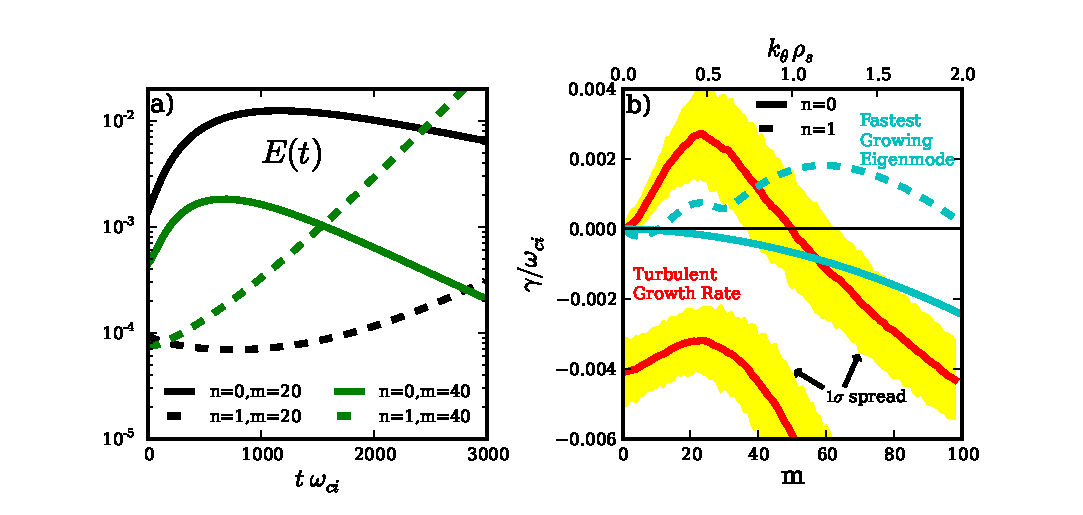
\includegraphics[width=0.55\textwidth]{n0_n1_growth}}
\caption{a) Linear evolution of energy starting from a turbulent initial state. The $n=0$ curves have an initial period of transient growth before exponentially decaying.
b) Linear and turbulent growth rate spectra for $n=0$ (solid lines) and $n=1$ (dashed lines) Fourier components. The linear growth rates are those of the least stable eigenmodes,
while the turbulent growth rates represent $\pdiff{E}{t}|_{\rm{lin}}/2 E$ from the nonlinear simulation. The shaded region marks the $1 \sigma$ spread in the turbulent spectrum,
obtained from the distribution of growth rates in the nonlinear simulation.}
\label{n0_n1_growth}
\end{figure}

This convective transport of density filaments is akin to the paradigmatic ``lift-up'' mechanism in hydrodynamic shear flows whereby streamwise vortices drive streamwise 
streaks~\cite{trefethen1993,krommes1999}.
Both are transient growth processes. We see this in our simulations by following the evolution of the energy of several $m,n$ modes after turning off the nonlinearities in an already
turbulent simulation. A few representative modes are shown in Fig.~\ref{n0_n1_growth} a). The linear transient growth of the filamentary $n=0$ structures is evident as their modes 
grow transiently before decaying exponentially at the rate of their least stable eigenmode. Such behavior is rather unituitive because all $n=0$ linear eigenmodes are stable, 
and the normal mode paradigm has conditioned us to believe that a linear superposition of such eigenmodes should decay. But as the hydrodynamics community discovered, linear
superpositions of nonorthogonal vectors may behave unintuitively.
Notice finally that the $n=1,m=20$ mode decays transiently before growing exponentially with growth rate of the most unstable eigenmode.
%This isn't necessarily due to eigenvector nonorthogonality, but is nevertheless unintuitive.

Since transient growth is a purely linear phenomenon, it has been a goal of researchers to predict the onset of subcritical turbulence using
only linear, non-modal calculations. It is our goal, however, to use linear calculations to go beyond predicting onset and predict fluctuation amplitudes and transport associated with saturated turbulence.
Perhaps one of the most useful statistical properties that we can predict is the turbulent growth rate spectrum.
To obtain a growth rate from the nonlinear simulation, we begin with the expression $\diff{E(m,n)}{t}\big|_{\rm{lin}} = Q(m,n) + D(m,n)$, 
which accounts for the total net energy injection into the fluctuations at each $m,n$. 
An effective growth rate $\gamma_e(m,n) = \diff{E(m,n)}{t}\big|_{\rm{lin}}/ 2 E(m,n)$ can then be defined. 
This growth rate is calculated from the spatial structure of the fluctuations, so it is well-defined for both turbulent fluctuations and eigenmode fluctuations. If calculated
from a linear simulation that is run for a sufficiently long time, $\gamma_e(m,n)$ is the same as the spectral eigenmode growth rate $\gamma_s(m,n)$ of the least stable linear eigenmode.
For turbulence, $\gamma_e(m,n)$ is generally not equal to an eigenmode growth rate, especially when the system is non-normal.
We plot this growth rate in Fig.~\ref{n0_n1_growth} b) for $n=0$ and $n=1$ components. The turbulent growth rate curves are calculated from this formula, 
averaged over a time of about $3 \times 10^{4} \ \omega_{ci}^{-1}$ during the saturated turbulent phase of the nonlinear simulation.
Also, we show the $1 \sigma$ contour, which indicates how greatly $\gamma_e$ varies over time.
Fig.~\ref{n0_n1_growth} b) indicates that while the linear eigenmodes are unstable for $n=1$ and stable for $n=0$,
the turbulent growth rates are positive for $n=0, m<50$ (subcritical-like behavior), but negative elsewhere. 
Fig.~\ref{n0_n1_growth} a) hinted at these characteristics, but this figure represents quantitative confirmation.

Our goal now is to reproduce the turbulent growth rate curves in Fig.~\ref{n0_n1_growth} b) without performing nonlinear simulations. 
To accomplish this, we use the anzatz that nonlinearities randomize the turbulent spatial structure at each wavenumber on a time scale of 
one eddy decorrelation time, while the linearities evolve the spatial structures deterministically. From this we can calculate a ``Transient Growth Rate'' spectrum,
which is our prediction of the turbulent growth rate spectrum. To illustrate,
we begin by taking Eqs.~\ref{ni_eq}-\ref{te_eq} and Fourier decomposing in the azimuthal and axial directions.  Then, we discritize in the radial direction and
approximate radial derivatives with finite differences.  The resulting system of equations may be written in matrix form:

\beqar
\label{mat_eq}
\mathbf{B}_{m,n} \diff{\mathbf{v}_{m,n}(t)}{t} = \mathbf{C}_{m,n} \mathbf{v}_{m,n}(t) \nonumber \\
- \sum_{m',n'}  \mathbf{v}_{E,m-m',n-n'} \cdot \gradperp \left( \mathbf{B}_{m',n'} \mathbf{v}_{m',n'}(t) \right),
\eeqar
where $\mathbf{v}_{m,n} = \left( N(r), \vpe(r), \phi(r), T_e(r) \right)_{m,n}^{T}$ is the state of the system,
and $\mathbf{B}_{m,n}$ and $\mathbf{C}_{m,n}$ are coefficient matrices that include the equilibrium information and finite difference coefficients. The first term on the RHS represents the linearities
and the second term the nonlinearities. Note that for each $m,n$, there exist $4 \times N_r$ linearly independent, but nonorthogonal eigenvectors. Hence forth, we drop the $m,n$ subscripts.

In order to use non-modal analysis to calculate growth rates and other measures, one must choose a norm and inner product with which to work. While any choice of
inner product is possible, a physically relevant one such as an energy inner product is generally preferred~\cite{camargo1998,schmid2007,camporeale2010}. 
Recall that the inner product of two vectors may be written $\left< \mathbf{x},\mathbf{y} \right> = \mathbf{y}^{*} \mathbf{M} \mathbf{x}$,
where $^*$ stands for the conjugate transpose, and $\mathbf{M}$ is a positive-definite matrix. We choose $\mathbf{M}$ so that 
$||\mathbf{v}|| = \sqrt{\left< \mathbf{v},\mathbf{v} \right>} = \sqrt{E}$, where $E$ is the energy. Furthermore, it is convenient in
computations to use the $L_2$-norm, $||\mathbf{u}||_2 = \sqrt{\sum_i |u_i|^2}$. This can be accomplished through the change of variables $\mathbf{u} = \mathbf{M}^{\frac{1}{2}} \mathbf{v}$.
Then the linear portion of Eq.~\ref{mat_eq} becomes

\beq
\label{lin_eq_A}
\diff{\mathbf{u}}{t} = \mathbf{A} \mathbf{u},  \quad \rm{where} \ \mathbf{A} = \mathbf{M}^{\frac{1}{2}} \mathbf{B}^{-1} \mathbf{C} \mathbf{M}^{-\frac{1}{2}}.
\eeq
%The eigenvalues of $\mathbf{A}$ are the same as those of $\mathbf{B}^{-1} \mathbf{C}$ because $\mathbf{M}^{\frac{1}{2}} \mathbf{B}^{-1} \mathbf{C} \mathbf{M}^{-\frac{1}{2}}$ is a similarity transformation.
The solution of Eq.~\ref{lin_eq_A} is $\mathbf{u}(t) = e^{\mathbf{A} t} \mathbf{u}(0)$, which
depends on the initial condition $\mathbf{u}(0)$ in addition to the spectral properties of $\mathbf{A}$. For purposes of turbulent growth rate prediction, we are interested in
the behavior of $||\mathbf{u}(t)||$. Therefore, we introduce the growth ratio $G(t)$, which measures the amplification or reduction in the square root of the energy from an initial state:

\beq
\label{g_def}
G(t) = \frac{||\mathbf{u}(t)||}{||\mathbf{u}(0)||} = \frac{||e^{\mathbf{A} t} \mathbf{u}(0)||}{||\mathbf{u}(0)||}.
\eeq
This ratio is bounded from above by $G_{\rm{max}}(t) = ||e^{\mathbf{A} t}||$. $G_{\rm{max}}(t) = e^{\gamma_s t}$ if and only if $\mathbf{A}$ is normal~\cite{schmid2007}. 
Otherwise, $G_{\rm{max}}(t) > e^{\gamma_s t}$. 

\begin{figure}
\centerline{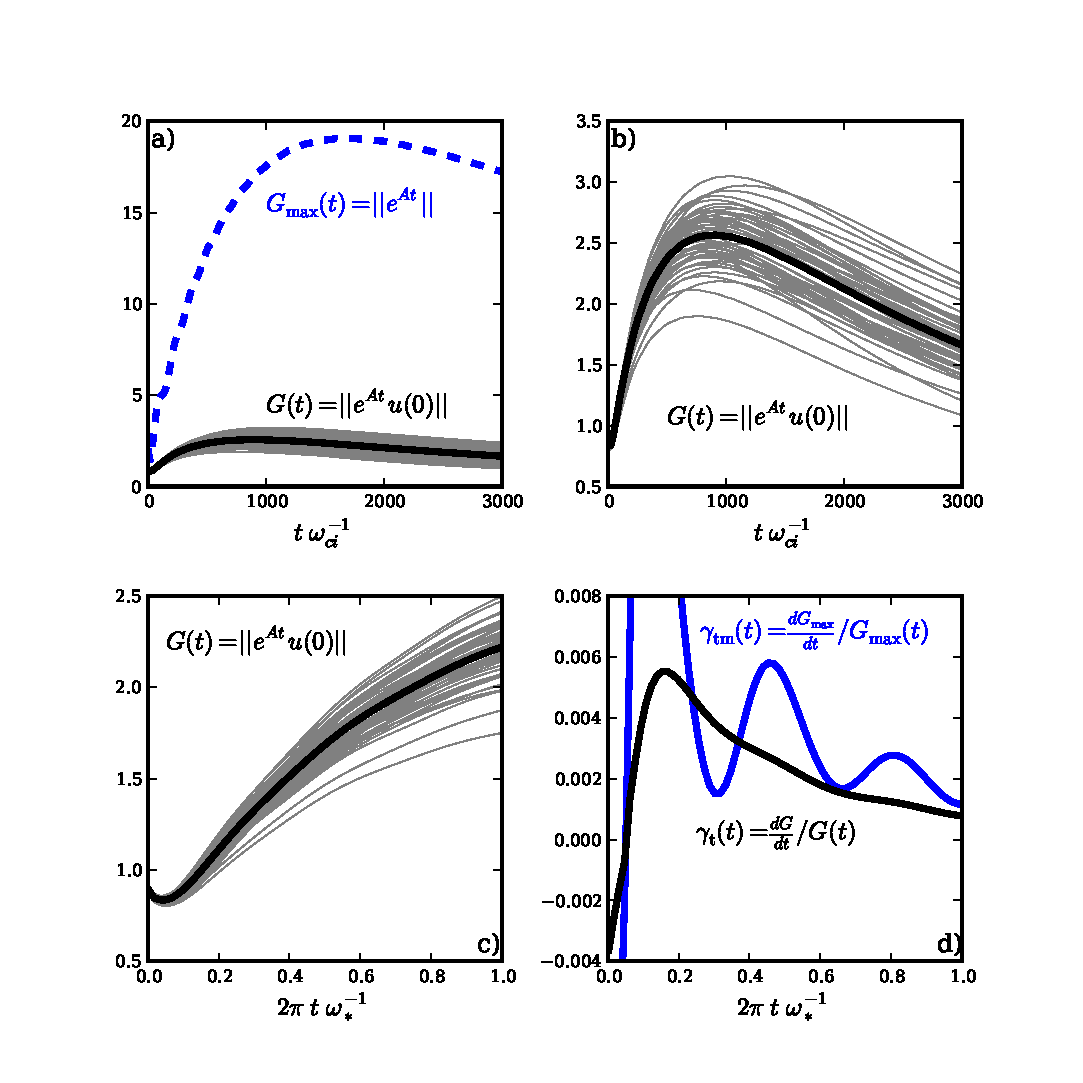
\includegraphics[width=0.55\textwidth]{m20n0_time_evs}}
\caption{a) The maximum growth ratio curve $G_{\rm{max}}(t)$ (dashed line) for $n=0,m=20$, and an ensemble of growth ratio curves (solid gray lines, with the solid black line the ensemble average)
that start with a random initial condition $u(0)$ and evolve under the linear operator. b) The ensemble curves with $t=\omega_s^{-1}$ indicated, at which we cut off the evolution.}
\label{m20n0_time_evs}
\end{figure}

It is common practice in normal mode analysis to look for the least stable eigenmode. 
For the non-modal case, it is common to study the properties of $G_{\rm{max}}(t)$ because if $G_{\rm{max}}(t) > 1$ at any time, fluctuations may be amplified, leading to subcritical turbulence.
However, it can be misleading to study only $G_{\rm{max}}(t)$ when predicting specific properties of turbulence because
$G_{\rm{max}}(t)$ is only the upper envelope of all possible $G(t)$ curves. No one particular initial condition $\mathbf{u}(0)$ evolves along $G_{\rm{max}}(t)$. 
Furthermore, it isn't obvious what kind of spatial structure or structures will come to dominate a turbulent system.
In non-normal systems, unlike in the normal systems, optimal structures don't amplify themselves, rather, they evolve while increasing the total fluctuating energy.

We illustrate $G_{\rm{max}}(t)$ along with $G(t)$ at $m=20, n=0$ for several random initial conditions in Fig.~\ref{m20n0_time_evs} a). Despite the fact that all eigenmodes at this
wavenumber are stable, there is the possibility for transient amplification by a factor of $20$. Furthermore, a sample of randomly initialized vectors are all transiently amplified, but none display
optimal growth. It is extremely unlikely to choose a random initial vector that either optimally amplifies the energy at any time or one that monotonically decays, which would be the case
if the initial vector were one of the linear eigenvectors. 

The key to quantifying non-modal analysis and making it predictive is to successfully model the effect that the nonlinearities have on the transient linear processes. 
To this effect, we note that the advective nonlinearity in Eq.~\ref{mat_eq} has the form of the state vector divided by a time $\tau_{\rm{nl}} \sim (v_E k_\perp)^{-1}$. This nonlinear
time scale is generally associated with the eddy turnover or decorrelation time. We therefore present a heuristic model of the nonlinearities 
as a randomizing force that acts on this characteristic nonlinear time scale.
Specifically, we start with a random initial condition, evolve it linearly for a time $\tau_{\rm{nl}}$, and then re-randomized the system.
To estimate $\tau_{\rm{nl}}$, we invoke the conjecture of \emph{critical balance}, which posits that the nonlinear time scale equals the linear time scale at all spatial scales~\cite{schekochihin2012}. 
For the linear time scale, we take the inverse of the linear frequency (at each $m,n$) -- $\tau_{\rm{nl}} = \omega_s^{-1}$.
However, $\omega_s = 0$ for $n=0$ linear eigenmodes, so we are forced to use $\omega_s$ for the fastest growing $n=1$ eigenmode at each $m$ to get a meaningful time scale. This is not wholly
unjustified, however, due to the inherent nonlinear coupling of different modes, evident in Eq.~\ref{mat_eq}.
In Fig.~\ref{m20n0_time_evs} b), this time scale is indicated. Note that we cut off the transient growth well before optimal amplification occurs, at least for this wavenumber.

We define the ``Transient Growth Rate'' $\gamma_{\rm{TR}}$ as the average from $t=0$ to $t=\omega_s^{-1}$ of the instantaneous growth rate of the ensemble averaged growth curve.
In Fig.~\ref{spec_nl_transient_gamma}, we compare the $\gamma_{\rm{TR}}$ spectrum (labeled ``Trans. $\omega_s^{-1}$'') to the turbulent spectrum.
Although the $\gamma_{\rm{TR}}$ spectrum for $n=0$ is downshifted in $m$ number relative to the spectrum derived from the nonlinear simulation, the two curves in Fig.~\ref{spec_nl_transient_gamma} a)
are fairly similar in shape and magnitude.
The $n=1$ curves in Fig.~\ref{spec_nl_transient_gamma} b), on the other hand, are not very similar, but $\gamma_{\rm{TR}}$ correctly predicts energy damping in the region where
eigenmode growth is predicted.
The difference between the $n=1$ transient and turbulent growth rate spectra is due to nonlinear effects not captured by the simple transient calculation procedure. In particular, the nonlinear
simulation has strong energy transfer from $n=0$ to $n=1$ which dissipates by electron-ion collisions~\cite{friedman2012b}. 

We include one more growth rate curve in Fig.~\ref{spec_nl_transient_gamma}, labelled ``Trans $\omega_s^{-1}$ cascade,'' to address the apparent downshift (in $m$) of
the ``Trans $\omega_s^{-1}$'' curve. As seen in Eq.~\ref{mat_eq}, $v_{m,n}$ is affected by every $\mathbf{v}_{E,m-m',n-n'} k^{'}_\perp$, not by only $\mathbf{v}_{E,m,n} k_\perp$ as we
assumed when using $\omega_s^{-1}$. Thus, we pose a simple forward cascade (eddy mitosis) model for the nonlinearity.
We use $\omega_s^{-1}$ at $m/2$ rather than $m$ for the randomizing time scale at each $m$ in deriving the ``Trans $\omega_s^{-1}$ cascade'' curves. 
The $n=0$ curve matches well with the $n=0$ Turbulent Growth Rate curve at $m>20$, but poorly for $m<20$ as expected since the cascade applies only at high $m$. 
We cannot determine \emph{a priori} the minimum $m$ for which the cascade should apply, so this method is not predictive.

\begin{figure}
\centerline{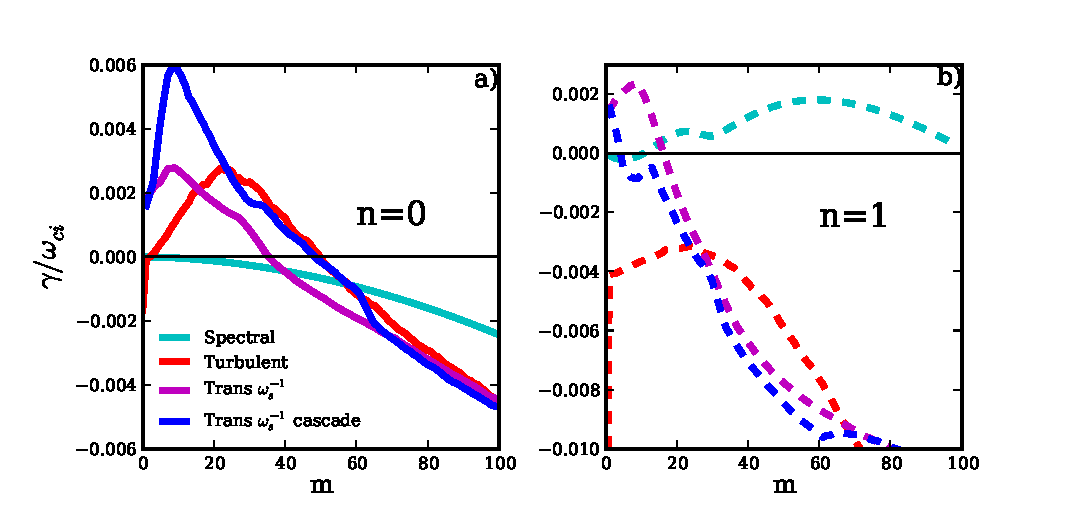
\includegraphics[width=0.5\textwidth]{spec_nl_transient_gamma}}
\caption{The linear, turbulent, and transient growth rate spectra. The transient spectra are calculated by the average growth rate over a time $\omega_s^{-1}(m,n=1)$ for the ensemble average
growth ratio curves with the cascade curve using $\omega_s^{-1}$ at $m/2$ rather than $m$.}
\label{spec_nl_transient_gamma}
\end{figure}

Nevertheless, our non-modal method, which requires only linear calculations, reproduces energetic growth properties of the turbulence not captured by eigenmode analysis.
Furthermore, when linear systems are highly non-normal, transient growth rates should be used in the kinds of predictions that are currently made with eigenmode growth rates. 
For instance, quasilinear theory uses the most unstable eigenmode growth rate $\gamma_{s,max}$ to predict the turbulent saturation levels using a mixing-length argument 
(saturated amplitude $\sim \gamma/k_\perp^2$). 
Using this formula with $\gamma_{s,\rm{max}} = 0.002$ and $m=60$, one predicts a turbulent saturation level of $\sim 0.1 \%$ which is wholly inconsistent with experiment and simulation. 
On the other hand, using this formula with the transient values $\gamma_{\rm{TR, max}} = 0.003, \ m=10$, we predict the saturation level of $\sim 10 \%$,
which is consistent with the nonlinear simulation and experimental measurements.

In summary, we present a procedure for predicting the turbulent growth rate spectrum using non-modal linear calculations. 
In the case of an LAPD experiment, this procedure captures the behavior of a nonlinear instability that dominates the dynamics of the turbulence.  In general,
non-modal initial-value analysis is difficult to quantify and make predictive, but using some simple nonlinear modelling, we have shown
that it is possible. Future studies will attempt to improve on the nonlinear modelling and expand the use of this technique to other non-normal turbulence models.  

This work was supported by the National Science Foundation (Grant PHY-1202007)

%%%%%%%%%%%%%%%%%%%%%%%%%%%%%%%%%%%%%%%%%%%%%%%%%%%%%%%%%%%%%%%%%%%%%%%%%%%

\bibliographystyle{phaip}
\bibliography{refs}


\end{document}
